\chapter{Studies in Constructed Memories}

\section{Introduction}

The memory of a conscious organism is a phenomenon in which 
interrelations of mind, language, and the rest of reality are especially evident. 
In these studies, I will define some conscious memory-systems, and 
investigate them. The investigation will be mathematical. In fact, the nearest 
precedent for it is perhaps the geometry of Nicholas Lobachevski. 
Non-Euclidian geometry had many founders, but Lobachevski in particular 
spoke of his system as an \enquote{imaginary geometry.} Lobachevski's system was, 
so to speak, the physical geometry of an \enquote{imaginary,} or constructed, space. 
By analogy, my investigation could be called a psychological algebra of 
constructed minds. It is too early to characterize the investigation more 
exactly. Let us just remember Rudoiph Carnap's \uline{Principle of Tolerance} in 
mathematics: the mathematician is free to construct his system in any way 
he chooses. 

I will begin by introducing a repertory of concepts informally, becoming more formal as I go along. Consider ongoing actions, which by definition extend through past, present, and future. For example, \enquote{I am making the trip from New York to Chicago.} Consider also past actions which have probable consequences in the present. \enquote{I have been heating this water} (entailing that it isn't frozen now). I will be concerned with such actions as these. 

Our language provides for the following assertion: \enquote{I am off to the country today; I could have been off to the beach; I could not possibly have been going to the center of the sun}. We distinguish an actual action from a possible action; and distinguish both from an action which is materially impossible. People insist that there are things they could do, even though they don't choose to do them (as opposed to things they couldn't do). What distinguishes these possible actions from impossible ones? Rather than trying to analyze such everyday notions in terms of the logic of counterfactual conditionals, or of modalities, or of probability, I choose to take the notions at their face value. My concern is not to philosophize, but to assemble concepts with which to define an interesting memory system. 

What is the introspective psychological difference between a thought 
that has the force of a memory, and a thought that has the force of a 
fantasied past, a merely possible past? I am not asking how I know that a 
verbalized memory is true; I am asking what quality a naive thought has that 
marks it as a memory. Let Alternative $E$ be that I went to an East Side 
restaurant yesterday, and Alternative $W$ be that I went to a West Side one. 
By the \enquote{thought of $E$} I mean mainly the visualization of going into the East 
Side restaurant. My thought of $E$ has the force of memory. It actually 
happened. $W$ is something I could have done. I can imagine I did do W. There 
is nothing present which indicates whether I did $E$ or $W$. Yet $W$ merely has 
the force of possibility, of fantasy. How do the two thoughts differ? Is the 
thought of $E$ involuntarily more vivid? Is there perhaps an \enquote{attitude of 
assertion} involuntarily present in the thought of $E$? 

Consider the memory that I was almost run down by a truck yesterday: 
I could have been run down, but wasn't. In such a case, the possibility that I 
could have been run down would be more vivid than the actuality that I 
wasn't. (Is it not insanity, when a person is overwhelmed by the fear of a 
merely possible past event?) My hold on sanity here would be the awareness 
that I am alive and well today. 

In dreams, do we not wholeheartedly \enquote{remember} that a misfortune 
has befallen us, and begin to adjust emotionally to it? Then we awake, and 
wholeheartedly remember that the misfortune has not befallen us. The 
thought that had the force of memory in the dream ceases to have that force 
as we awake. We remember the dream, and conclude that it was a fantasy. 
Even more characteristic of dreams, do I not to all intents and purposes go 
to far places and carry out all sorts of actions in a dream, only to awaken in 
bed? We say that the dream falsifies my present environment, my 
sensations, my actions, memories, the past, my whole world, in a totally 
convincing way. Can a hypnotist produce artificial dreams, that is, can he 
control their content? Can the hypnotist give his subject one false memory 
one moment, and replace it with a contradictory memory the next 
moment? 

I will now specify a situation involving possible actions and 
remembering. 

\newenvironment{hangers}{\vskip 0.5em\begin{hangparas}{3em}{1}}{\end{hangparas}\vskip 0.5em}

\begin{hangers}
\textbf{Situation 1.} \enquote{I could have been accomplishing $G$ by doing $A_{a_1}$, or by 
doing $A_{a_2}$, \ldots, or by doing $A_{a_n}$; but I have actually been accomplishing $G$ by 
doing $A_{a_1}$.} Here the ongoing actions $A_{a_i}$, $i=1,\ldots,n$,$a_i\neq a_h$ if $i\neq h$, are 
the possible methods of accomplishing $G$. (The subscripts are supposed to 
indicate that the methods are distinct and countable, but not ordered.) The 
possible methods cannot be combined, let us assume. 
\end{hangers}

In such a situation, perhaps the thought that I have been doing $A_{a_1}$
would be distinguished from similar thoughts about $A_{a_2}, \ldots, A_{a_n}$ by the
presence of the \enquote{attitude of assertion}. Since the possible methods are 
ongoing actions, the thought that I have been doing $A_{a_i}$ has logical or 
probabie consequences I can check against the present. 

Now $A_{a_1}$, is actual and $A_{a_2}$ is not, so that $A_{a_1}$, simply cannot have 
possible jar in $A_{a_3}$ to contain it. The only \enquote{connection} $A_{a_1}$ could have
material contact with $A_{a_2}$. An actual liquid in $A_{a_1}$ could not require a 
with $A_{a_2}$, would be verbal and gratuitous. Therefore, in order to be possible 
methods, $A_{a_2}$, \ldots, $A_{a_n}$ must be materially separable. A liquid in $A_{a_2}$ must
not require a jar in $A_{a_3}$ to contain it. If it did, $A_{a_2}$ couldn't be actualized 
while $A_{a_3}$, remained only a possibility. 

Enough concepts are now at hand for the studies to begin in earnest. 

\section{M-Memories}

\newcommand{\definition}{\textbf{Definition.}}
\newcommand{\assumption}[1]{\textit{Assumption #1.}}
\newcommand{\conclusion}[1]{\textbf{Conclusion #1.}}

\begin{hangers}
\definition\ Given the sentences \enquote{I have actually been doing $A_{a_i}$}, where 
the $A_{a_i}$ are non-combinable possible methods as in Situation 1, an 
\enquote{M-Memory} is a memory of a conscious organism such that the organism 
can think precisely one of the sentences at a time, and any of the sentences 
has the force of memory. 
\end{hangers}

This definition refers to language, mind, and the rest of reality in their 
interrelations, but the crucial reference is to a property of certain sentences. 
I have chosen this formulation precisely because of what I want to 
investigate. I want to find the minimal, elegant, extra-linguistic conditions, 
whatever they may be, for the existence of an M-Memory (which is defined 
by a linguistic property). I can say at once that the conditions must enable 
the organism to think the sentences at will, and they must provide that the 
memory is consistent with the organism's present awareness. 

\begin{hangers}
\definition\ The \term{P-Memory} of a conscious organism is its conscious 
memory of what it did and what happened to it, the past events of its life. I 
want to distinguish here the \enquote{personal} memory from the preconscious. 

\definition\ An \term{L-Memory} is a linguistic P-Memory having no 
extra-linguistic component. Of course, the linguistic component has 
extra-linguistic mental associations which give it \enquote{meaning}--otherwise the 
memory wouldn't be conscious. But these associations lack the force of a 
mental reliving of the past independent of language. An L-Memory amounts 
to extra-linguistic amnesia. 

\assumption{1.1} With respect to normal human memory, when I forget 
whether I did $x$, I can't voluntarily give either the thought that I did $x$, or 
the thought that I didn't do $x$, the force of memory. I know that I either did 
or didn't do $x$, but I can create no conviction for either alternative. (An 
introspective observation.) 

\conclusion{1.2} An L-Memory is not sufficient for an M-Memory, even 
in the trivial case that the $A_{a_i}$ are beyond perception (as internal bodily 
processes are). True, there would be no present perceptions to check the 
sentences \enquote{I have actually been doing $A_{a_i}$} against. True, the L-Memory 
precludes any extra-linguistic memory-\enquote{feelings} which would conflict with 
the sentences. But the L-Memory is otherwise normal. And \textit{Assumption 1.1}
indicates that normally, either precisely one of a number of mutually 
exclusive possibilities has the force of memory; or else the organism can give 
none of them the force of memory. 

\assumption{1.3} I cannot, from within a natural dream, choose to swith 
to another dream. (An introspective observation. A \enquote{natural} dream is a 
dream involuntarily produced internally during sleep.) 

\conclusion{1.4} An M-Memory could not be produced by natural 
dreaming. It is true that in one dream one sentence could have the force of 
memory, and in another dream a different sentence could. But an M-Memory 
is such that the organism can choose one sentence-memory one moment and 
another the next. See Assumption 1.3. 

\assumption{1.5} Returning to the example of the restaurants, I find 
that months after the event, my thought of $E$ no longer has the force of 
memory. All I remember now is that I used to remember that I did $E$. I 
remember that I did $E$ indirectly, by remembering that I remembered that I 
did $E$. (My memory that I did $E$ is becoming an L-Memory.) The assumption 
is that a memory of one's remembering can indicate, if not imply, that the 
event originally remembered occurred. 

\conclusion{1.6} The following are adequate conditions for the existence 
of an M-Memory. 
\begin{enumerate}
\item The sentences are the organism's only memory of which 
method he has been using. 

\item When the organism thinks \enquote{I have actually been doing $A_{a_i}$}.
then (he artificially dreams that) he has been doing $A_{a_i}$ --- and is 
now doing it. 

\item When the dream ends, he does not remember that he 
remembered that \enquote{he has been doing $A_{a_i}$,} That is, he does not remember 
the dream; and he does not remember that he thought the sentence. These 
conditions would permit the existence of an M-Memory or else a memory 
indistinguishable to all intents and purposes from an M-Memory. 
\end{enumerate}
\end{hangers}

What I have in mind in \conclusion{1.6} is dreams which are produced 
artificially but otherwise have all the remarkable qualities of natural dreams. 
There would have to be a state of affairs such that the sentence would 
instantly start the dream going. 

So much for the conditions for the existence of an M-Memory. 
Consider now what it is like as a mental experience to have an M-Memory. 
What present or ongoing awareness accompanies an M-Memory? 
\conclusion{1.6.2} already told what the remembering is like. For the rest, I will 
informally sketch some conclusions. The organism can extra-linguistically 
image the $A_{a_i}$. The organism can think \enquote{I could have been doing $A_{a_i}$.} When 
not remembering, the organism doesn't have to do any $A_{a_i}$, or he can do any 
one of them. The organism must not do anything which would liquidate a 
possble method, render the action no longer possible for him. 

\begin{hangers}
\assumption{2.1} A normal dream can combine two totally different 
past episodes in my life into a fused episode, or amalgam; so that I \enquote{relive} it 
without doubts as.a single episode, and yet remain vaguely aware that 
different episodes are present in it. Dreams have the capacity not only to 
falsify my world, but to make the impossible believable. (An introspective 
observation.) 

\conclusion{2.2} The conditions for the existence of an M-Memory 
further permit material contact between the possible methods, the very 
contact which is out of the question in a normal Situation 1. The dream is so 
flexible that the organism can dream that an (actual) liquid is\slash was contained 
by a jar in a possible method. See \assumption{2.1} Thus, the $A_{a_i}$ do not have 
to be separable to be possible methods. 
\end{hangers}

I will now introduce further concepts pertaining to the mind. 

\begin{hangers}
\definition\ A \term{mental state} is a mental \enquote{stage} or \enquote{space} or \enquote{mood} 
in which visualizing, remembering, and all imaging can be carried on. 
\end{hangers}

Some human mental states are stupor, general anxiety, empathy with 
another person, dizziness, general euphoria, clearheadedness (the normal 
state in which work is performed), and dreaming. In all but the last state, 
some simple visualization routine could be carried out voluntarily. Even ina 
dream, I can have visualizations, although here I can't have them at will. The 
states are not defined by the imaging or activities carried on while in them, 
but are \enquote{spaces} in which such imaging or activities are carried on. 

By definition. 

\begin{hangers}
\conclusion{3.2} An M-Memory has to occur within the time which the 
possible methods require, the time required to accomplish G. By definition. 

\definition\ An \term{M*-Memory} is an M-Memory satisfying these 
conditions. \label{mstardef}
\begin{enumerate}
\item $A_{a_i}$, for the entire time it requires, involves the voluntary 
assuming of mental states. $i=1,...,n$.
\item The material contact between the 
possible methods, the cross-method contact, is specifically some sort of 
contact between states. 
\end{enumerate}

\conclusion{3.3} For an M*-Memory, to remember is to choose the 
mental state in which the remembering is required to occur (by the 
memory). After all, for any M-Memory, to remember is to choose all the 
$A_{a_i}$-required things you are doing while you remember. 
\end{hangers}

By now, the character of this investigation should be clearer. I seek to 
stretch our concepts, rather that to find the \enquote{true} ones. The investigation 
may appear similar to the old discipline of philosophical psychology, but its 
thrust is rather toward the modern axiomatic systems. The reasoning is 
loose, but not arbitrary. And the investigation will become increasingly 
mathematical. 


\section{D-Memories}

\begin{hangers}
\definition\ A \term{D-Memory} is a memory such that measured past time 
	appears in it only in the following sentences: \enquote{$Event_j$ occurred in the interval 
% TODO\<F11><F12> ? whats up with AF
of time which is $x_j-x_{j-1}$ long and ended at $x_j$ $AF$, and is $y_j$ long and ended $z_j$
\ ago,} where $x_j$, $y_j$ and $z_j$ are positive numbers of time units (such as hours) 
and \enquote{$AF$} means \enquote{after a fixed beginning time.} $x_O=O;$ $x_j> x_{j-1}$; and at any 
one fixed time, the intervals $|z_j, z_j+y_j|$ nowhere overlap. $y_j+z_j\leq x_j$ For an
integer $m$, the $m$th sentence acquires the force of memory, is added to the 
memory, at the fixed time $x_m$. $j=1, \ldots, f(t)$, where the number of sentences 
$f(t)$ is written as a function of time $AF$. Then $f(t)=m$ when $x_m \leq t \less x_{m+1}$. 
The sentences have the force of memory involuntarily. The organism does 
not make them up at will. 
\end{hangers}

Let me explain what the D-Memory involves. $Event_j$ is assigned to an 
abnormal \enquote{interval,} a dual interval defined in two unrelated ways. The 
intervals defined by the $y_j$ and $z_j$ are tied to the present instant rather than to 
a fixed time, and could be written $|N-z_j-y_j, N-z_j|$, where '$N$' means "the time 
of the present instant relative to the fixed beginning time." 

\newcommand{\proof}{\textit{Proof}}

\begin{hangers}
\conclusion{4} The intervals $|N-z_j-y_j, N-z_j|$ nowhere overlap. 

\proof: By definition, the intervals $|z_j, z_j+y_j|$ nowhere overlap. If $j\neq k$,
$|z_j, z_j+y_j|\cap|z_k, z_k+y_k|=\emptyset$ 
This fact implies that e.g. $z_j\less z_j+y_j\less z_k\less z_k+y_k$.
Then $N-z_k-y_k\less N-z_k\less N-z_j-y_j\less N-z_j$.
Then $|N-z_k-y_k, N-z_k|\cap|N-z_j-y_j, N-z_j|=\emptyset$
At any one time, the organism can think of all the sliding intervals, and they 
partly cover the time up to now without overlapping. 
\end{hangers}

Suppose you find the deck of $n$ cards 

{ \centering {\vskip 1em}
	\framebox[1.1\width]{
		\parbox{1in}{
			\centering
			\large $event_{j}$ 
			{\vskip 0.25em}
			$z_{j}$ ago
		}
	}
	\par {\vskip 0.5em}
}



($j=1,\ldots,n$ and $z_j$ is a positive number of days), and you have no 
information to date them other than what they themselves say. If you 
believe the cards, your mental experience will be a little like having a 
D-Memory. Then, the definition does not require that $y_j=x_j-x_{j-1}$. Again, it is 
not that two concepts of \enquote{length} are involved, but that the \enquote{interval} is 
abnormal. Of course this is all inconsistent, but I want to study the 
conditions under which a mind will accept inconsistency. 

\begin{hangers}
\assumption{5.1} With respect to normal human memory, it is possible 
to forget what day it is, even though one remembers a past date. (An 
empirical observation.) 

\assumption{5.2} This assumption is based on the fact that the sign 
\enquote{\textsc{Closed for Vacation. Back in two weeks.}} was in the window of 
a nearby store for at least a month this summer; and the fact that a 
filmmaker wrote in a newspaper, \enquote{When an actor asks me when the film will 
be finished, I say \enquote{In two months,} and two months later I give the same 
answer, and I'm always right.} Even in normal circumstances, humans can 
maintain a dual and outright inconsistent awareness of measured time. In 
general, inconsistency is a normal aspect of human thinking and even has 
practical value. 
\end{hangers}

Imagine a child who has been told to date events by saying, for 
example, $x$ happened two days ago, and a day later saying again, $x$ happened 
two days ago---and who has not been told that this is inconsistent. What 
conditions are required for the acceptance of this dating system? It is 
precisely because of Assumptions 5.1 and 5.2 that a certain answer cannot 
be given to this question. The human mind is so flexible and malleable that 
there is no telling how much inconsistency it can absorb. I can only study 
what flaws might lead the child to reject the system. The child might \enquote{feel} 
that an event recedes into the past, something the memory doesn't express. 
An event might be placed by the memory no later than another, and yet 
\enquote{feel} more recent than the other. I speculate that if anything will discredit 
the system, it will be its conflict with naive, \enquote{felt,} extra-linguistic memory. 

\begin{hangers}
\conclusion{5.3} The above dating system would be acceptable to an 
organism with an L-Memory. 

\conclusion{5.4} The existence of an L-Memory is an adequate condition 
for the existence of a D-Memory. With extra-linguistic amnesia, the 
structure of the language would be the structure of the past in any case. The 
past would have no form independent of language. Anyway, time is gone for 
good, leaving nothing that can be checked directly. Without an 
extra-linguistic memory to fall back on, and considering Assumptions 5.1 
and 5.2, the dual temporal memory shouldn't be too much to absorb. 
\end{hangers}

As I said, the real difficulty with this line of investigation is putting 
limits on anything so flexible as the mind's capacity to absorb inconsistency. 

Now the thinking of a sentence in a D-Memory itself takes time. Let 
$\delta(S^D_j)$ be the minimum number of time units it takes to think the jth 
D-sentence. This function, abbreviated '$\delta_j$', is the duration function of the 
D-sentences. 

\begin{hangers}
\conclusion{6.1} If $\delta_j\greater z_j$, the memory of the interval defined by $y_j$ and 
$z_j$ places the end of the interval after the beginning of the memory of it, or 
does something else equally unclear. If $\delta_j\greater y_j+z_j$, the entire interval is placed 
after the beginning of the memory of it. When $\delta_j\greater z_j$, let us say that the end 
of the remembered interval falis within the interval for the memory of it, or 
that the situation is an \enquote{infall.} (Compare \enquote{The light went out a half-second 
ago}.)

\conclusion{6.2} If $\delta_j\greater x_{j+k}-x_j$, then $S^D_{j+k}$ is added to the preconscious 
	before $S^D_j$ can be thought once. The earliest interval during which the $j^{th}$ 
	sentence can be thought \enquote{passes over} the $(j+k)^{th}$ interval. Let us say that 
the situation is a \enquote{passover.} (Something of the sort is true of humans, 
whose brains contain permanent impressions of far more sensations than can 
be thought, remembered in consciousness.) 

\conclusion{6.3} If there are passovers in a D-Memory, the organism 
cannot both think the sentences during the earliest intervals possible and be 
aware of the passovers. 

\proof: The only way the organism can be aware of $\delta(S_j)$
is for $event_{j+h}$ ($h$ a positive integer) to be the thinking of $S_j$. 
If the thinking of $S_j$ takes piace as the $(j+1)^{th}$ event, then the organism gets two 
values for $\delta(S_j)$, namely $x_{j+1}-x_j$ and $y_{j+1}$. Assume that only $x_{j+1}-x_j$
is allowed as a measure of $\delta(S_j)$. Since $\delta(S_j)=x_{j+1}-x_j$, there is no passover. If 
the thinking of $S_j$ takes place as the $(j+2)^{th}$ event, then $x_{j+2}-x{j+1}=\delta(S_j)$
could be greater than $x_{j+1}-x_j$. But since $S_j$ goes into the preconscious at $x_j$, 
$S_j$ is not actually thought in the earliest interval during which it could be 
thought. See diagram \ref{dmemdiag}.

\begin{figure}
	\centering
	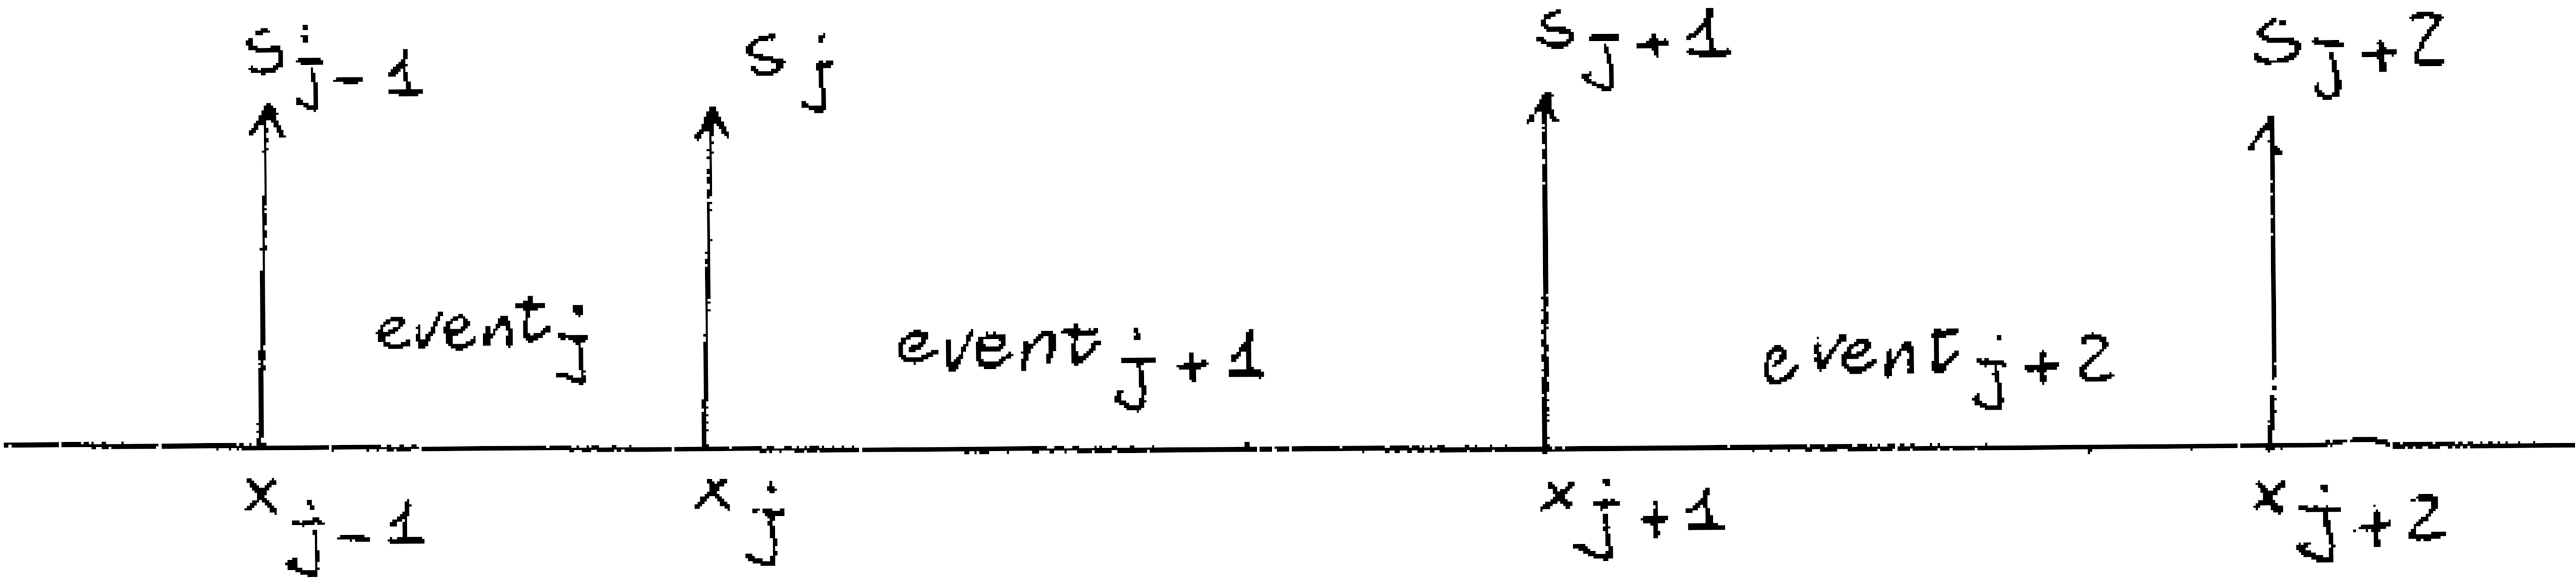
\includegraphics[width=4in]{img/dmemdiag}
	\caption{tktk}
	\label{dmemdiag}
\end{figure}

\conclusion{6.4} Let there be an \term{infall} in the case where $event_{j+1}$ is the 
thinking of $S_j$. $\delta(S_j)=x_{j+1}-x_j$ and $\delta(S_j)\greater z_j$. $S_{j+1}$ gives $\delta(S_j)$, 
so that the organism can be aware of it. 
It is greater than $z_j$. Thus, the organism can be 
aware of the infall. However, the infall will certainly be no more difficult to 
accept than the other features of the D-Memory. And the thinking of $S_j$ has 
to be one of the events for the organism to be aware of the infall. 
\end{hangers}

\section{$\Phi$-Memories}
I will conclude these studies with two complex constructions. 

\begin{hangers}
\definition\ A \enquote{$\Phi$-Memory} is a memory which includes an M*-Memory 
and a D-Memory, with the following conditions. 
\begin{enumerate}
\item The goal $G$, for the M*-Memory, is to move from one point to another. 

\item For the D-Memory, \enquote{$event_j$} becomes a numerical term, the decrease in the organism's distance 
from the destination point during the temporal interval. \enquote{A 3-inch move 
toward the destination} is the sort of thing that \enquote{$event_j$} here refers to. 

\item The number of $A_{a_i}$ equals the number of D-sentences factorial. The number 
of D-sentences, of course, increases. 
\end{enumerate}
\end{hangers}

Consider the consecutive thinking of each D-sentence precisely once, in 
minimum time, while the number of sentences remains constant. Such a 
\enquote{D-paragraph} is a permutation of the D-sentences. Let $\mathparagraph^m$ be a 
D-paragraph when the number of sentences equals the integer m. There are 
$m!$ $\mathparagraph^m$s. When $f(t)=m=3$, one of the six $\mathparagraph^3$s is $S^D_3 S^D_1 S^D_2$, 
thought in 
minimum time. Assume that the duration $\triangle$ of a D-paragraph depends only 
on the number of D-sentences and the $\delta_j$. We can write 

$$ \triangle(\mathparagraph^m)=\sum_{j=1}^{m} \delta_j $$

The permutations of the D-sentences, as well as the D-paragraphs, can be 
indexed with the $a_i$, just as the possible methods are. 

\begin{hangers}
\definition\ A \enquote{$\Phi^*$-Memory} is a $\Phi$-Memory in which the order of the 
sentences in the $a_i$th $\mathparagraph^m$ has the meaning of \enquote{I have actually been doing $A_{a_i}$}
assigned to it. The order is the indication that $A_{a_i}$ has actually been used; it 
is the $a_j$th $M^*$-assertion. \enquote{I have actually been doing $A_{a_i}$} is merely an English 
translation, and does not appear in the $\Phi^*$-Memory. 

\conclusion{7} Given a $\Phi^*$-Memory, if one D-sentence is forgotten, not 
only will there be a gap in the awareness of when what events occurred; it 
will be forgotten which method has actually been used. 
\end{hangers}

This conclusion points toward a study in which deformations of the 
memory language are related to deformations of general consciousness. 

\begin{hangers}
\definition\ A \enquote{$\Phi^*$-Reflection,} or reflection in the present of a 
$\Phi^*$-Memory, is a collection of assertions about the future, derived from a 
$\Phi^*$-Memory, as follows. 
\begin{enumerate}
	\item There are the sentences \enquote{$Event_j$ will occur in the 
interval of time which is $x_j-x_{j-1}$ long, and begins at twice the present time 
$AF$, minus $x_j AF$; and which is $y_j$ long and begins $z_j$ from now.} If $event_j$ was 
		a 3-inch move toward the destination in the \enquote{$\Phi^*$-Memory,} the sentence in the 
$\Phi^*$-Reflection says that a 3-inch move will be made in the future temporal 
interval. 
	\item The $a_i$th permutation of the sentences defined in (1) is an 
assertion which has the meaning of \enquote{I will do $A_{a_i}$}; and the organism can 
think precisely one permutation at a time. The $A_{a_i}$, $x_j$, $y_j$, $z_j$, and the rest are 
defined as before (so that in particular the permutations can be indexed with 
the $a_i$). 
\end{enumerate}
\end{hangers}
\begin{hangers}
\conclusion{8} Given that the $\Phi^*$-Memory's temporal intervals $|x_{j-1}, x_j|$
are reflected as $|2N-x_j, 2N-x_{j-1}|$, the reflection preserves the intervals' 
absolute distances from the present. 

\proof: The least distance of $|x_{j-1}, x_j|$
from $N$ is $N-x_j$; the greatest distance is $N-x_{j-1}$. Adding the least distance, and 
then the greatest distance, to $N$, gives $|2N-x_j, 2N-x_{j-1}|$.
\end{hangers}

I will end with two problems. If a $\Phi^*$-Memory exists, under what 
conditions will a $\Phi^*$-Reflection be a precognition? Under what conditions 
will every assertion be prescience or foreknowledge? By a \enquote{precognition} I 
don't mean a prediction about the future implied by deterministic laws; I 
mean a direct \enquote{memory} of the future unconnected with general principles. 

Finally, what would a precognitive $\Phi^*$-Reflection be like as a mental 
experience? What present or ongoing awareness would accompany a 
precognitive $\Phi^*$-Reflection? 

